% \documentclass{report}
% \usepackage{fancyhdr}
\usepackage{fourier-orns}
\usepackage{hyperref}%% To refrence links / jumps
\usepackage{chngcntr} %% For some extra counters numberings
\usepackage[a4paper, right = 0.5in, left = 0.5in,top = 1in , bottom = 1in]{geometry}
\usepackage{etoolbox} %% Provides like a language for advanced customization
\usepackage{datetime} %% For dates of course
\usepackage{lastpage} %% provides pages numbers
\usepackage[sc]{titlesec} %% modify titles
\usepackage{enumerate}
\usepackage{cancel}
\usepackage{tikzsymbols}
\usepackage[dvipsnames]{xcolor}
\usepackage{import}
\usepackage{pdfpages} %% include other pdfs
\usepackage{transparent} %% Transparency
\usepackage{xcolor}  %% Colors
\usepackage[many]{tcolorbox}
\usepackage[framemethod=TikZ]{mdframed}
\usepackage{amsmath,amsfonts,amsthm,amssymb,mathtools}
\usepackage{tikz}
\usepackage{bookmark}
\usepackage{graphicx}
\usepackage{mathpazo}

\usepackage{fontawesome5}

\linespread{1.5}


\titleformat{\chapter}[display]   
{\fontfamily{ppl}\selectfont\huge\color{YellowOrange!80!orange}} % Font style and size 
{\raggedleft\color{purple}\fontsize{70}{0pt}\selectfont\thechapter}   
{-1.5cm}    			                          % Space between the chapter number and title
{
	\begin{tikzpicture}[overlay]
		\node[anchor = west,yshift = 0.2cm,xshift = -1cm] {\fontsize{90}{20} $\int_{}^{} $};
		\node[yshift = 4cm, xshift = 17cm]   {\includegraphics[width = 4cm]{preview0}};
	\end{tikzpicture}
\hspace{1cm}\Huge\raggedright\MakeUppercase}

\titleformat{\section}[block]
{
\fontfamily{ppl}\selectfont\huge\color{YellowOrange!80!orange}
}
{
\color{purple}\fontsize{20}{0pt}\selectfont\thesection 
}
{0cm}
{
	\begin{tikzpicture}[overlay]
		\node[anchor = west,yshift = 0.2cm,xshift = -0.4cm, circle = 1pt] {};
	\end{tikzpicture}
}

\titlespacing*{\section}{0pt}{0.7cm}{1.5cm}


\newcommand{\divider}
{
	\begin{center}
	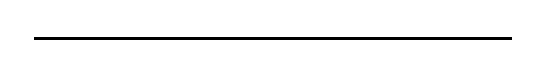
\begin{tikzpicture}
		\draw[thick, black] (0.25*\textwidth, 0) -- (0.75*\textwidth, 0);
		\node[rotate = 360 - 90, xshift = -0.6pt, yshift = 1pt] at (0.25*\textwidth,0){\decotwo};
		\node[rotate = 90, xshift = -0.6pt, yshift = 1pt] at (0.75*\textwidth,0){\decotwo};
	\end{tikzpicture}
	\end{center}
}

\pagestyle{fancy}

\newcommand{\lecday}[1][]
{
    \def\datee{#1}
    \fancyhead[L]{\datee}
}



\newcommand{\signature}
{
	\begin{tikzpicture}[remember picture,overlay]
		\node[fill = YellowOrange!20!white] at ([yshift = 1cm, xshift = -3cm]current page.south east) {\fontsize{10pt}{0pt}{\itshape Kara.$\mathcal{A}$}};
	\end{tikzpicture}
}

\AddToHook{shipout/background}{
  \begin{tikzpicture}[remember picture, overlay]
	  \node[] at ([yshift = 1.5cm,xshift = \textwidth /2 + 0.9cm]current page.south west) {\includegraphics[width = 0.5cm]{preview3}};
	  \node[] at ([yshift = 1.5cm,xshift = - \textwidth /2 - 0.9cm]current page.south east) {\includegraphics[width = 0.5cm]{preview4}};
  \end{tikzpicture}
}



\newtcolorbox[auto counter, number within = section]{remark}[1][]
{
       		title = Remark #1,
		enhanced,
		boxrule = 0pt,
		colback = white,
		breakable,
		arc = 4pt,
		colbacktitle = cyan,
		colback = cyan!5!white,
		segmentation style =
		{
			solid,cyan,thick,
		},
		attach boxed title to top left =
		{
			xshift = 0cm,
		},
		boxed title style =
		{
			boxrule = 0pt,
			sharp corners,
			drop fuzzy shadow = {cyan},
		},
		drop fuzzy shadow = {cyan!80!black},
}

\newtcolorbox[auto counter, number within = section]{theorem}[1][]
{                                      
		title = Theorem \thetcbcounter : #1,
		enhanced, 
		boxrule = 0pt,
		colback = white,
		breakable,
		arc = 4pt,
		colbacktitle = purple,
		colback = purple!5!white,
		segmentation style = 
		{
			solid, purple,thick,
		},
		attach boxed title to top left = 
		{
			xshift = 0cm, 
		},
		boxed title style = 
		{
			boxrule = 0pt,
			sharp corners,
			drop fuzzy shadow = {purple},
		},
		drop fuzzy shadow = {purple!80!black},
}

\newtcolorbox[auto counter, number within = section]{definition}[1][]
{                                      
		title = Definition \thetcbcounter : #1,
		enhanced, 
		boxrule = 0pt,
		colback = white,
		arc = 4pt,
		breakable,
		colbacktitle = YellowOrange!80!black,
		segmentation style = 
		{
			solid, YellowOrange,thick,
		},
		attach boxed title to top left = 
		{
			xshift = 0cm, 
		},
		colback = YellowOrange!5!white,
		boxed title style = 
		{
			boxrule = 0pt,
			sharp corners,
			drop fuzzy shadow = {YellowOrange!80!orange},
		},
		drop fuzzy shadow = {YellowOrange!80!black},
}

\newtcolorbox[auto counter, number within = section]{corollary}[1][]
{                                      
		title = corollary \thetcbcounter : #1,
		enhanced, 
		boxrule = 0pt,
		colback = white,
		arc = 4pt,
		breakable,
		colbacktitle = YellowOrange!80!black,
		segmentation style = 
		{
			solid, YellowOrange,thick,
		},
		attach boxed title to top left = 
		{
			xshift = 0cm, 
		},
		colback = YellowOrange!5!white,
		boxed title style = 
		{
			boxrule = 0pt,
			sharp corners,
			drop fuzzy shadow = {YellowOrange!80!orange},
		},
		drop fuzzy shadow = {YellowOrange!80!black},
}


\newtcolorbox{example}[1][]
{                                      
		title = Example,
		enhanced, 
		boxrule = 0pt,
		colback = white,
		arc = 4pt,
		segmentation style = 
		{
			solid, SpringGreen,thick,
		},
		breakable,
		colback = SpringGreen!5!white,
		colbacktitle = SpringGreen!80!black,
		attach boxed title to top left = 
		{
			xshift = 0cm, 
		},
		boxed title style = 
		{
			boxrule = 0pt,
			sharp corners,
			drop fuzzy shadow = {SpringGreen!80!orange},
		},
		drop fuzzy shadow = {SpringGreen!80!black},
}


\newcommand{\integral}[4]{\int\limits_{#1}^{#2} #4 d#3}
\newcommand{\limit}[3]{\lim\limits_{#1 \rightarrow #2} #3}
\newcommand{\strone}[2]{\left[ \begin{gathered}#1\\ #2\end{gathered} \right] }
\newcommand{\strtwo}[2]{\left\{ \begin{gathered}#1\\ #2\end{gathered} \right\} }
\newcommand{\strthree}[2]{\left\lfloor \begin{gathered}#1\\ #2\end{gathered} \right\rfloor }


\newcommand{\startbf}[1]{\text{\bfseries{#1}}}
\newcommand{\sett}[1]{\left\{ #1 \right\}}
\newcommand{\thesis}[1]{\left( #1 \right)}
\newcommand{\brkt}[1]{\left[ #1 \right]}
\newcommand{\floor}[1]{\left\lfloor #1 \right\rfloor}


\DeclareMathOperator{\img}{im} % Image
\DeclareMathOperator{\Img}{Im} % Image
\DeclareMathOperator{\coker}{coker} % Cokernel
\DeclareMathOperator{\Coker}{Coker} % Cokernel
\DeclareMathOperator{\Ker}{Ker} % Kernel
\DeclareMathOperator{\rank}{rank}
\DeclareMathOperator{\Spec}{Spec} % spectrum
\DeclareMathOperator{\Tr}{Tr} % trace
\DeclareMathOperator{\pr}{pr} % projection
\DeclareMathOperator{\ext}{ext} % extension
\DeclareMathOperator{\pred}{pred} % predecessor
\DeclareMathOperator{\dom}{dom} % domain
\DeclareMathOperator{\ran}{ran} % range
\DeclareMathOperator{\Hom}{Hom} % homomorphism
\DeclareMathOperator{\Mor}{Mor} % morphisms
\DeclareMathOperator{\End}{End} % endomorphism


\newcommand{\lm}{\ensuremath{\lambda}}
\newcommand{\eps}{\ensuremath{\epsilon}}
\newcommand{\veps}{\ensuremath{\varepsilon}}
\newcommand{\al}{\ensuremath{\alpha}}
\newcommand{\bb}{\ensuremath{\beta}}
\newcommand{\cc}{\ensuremath{\gamma}}
\newcommand{\dd}{\ensuremath{\delta}}
\newcommand{\DD}{\ensuremath{\Delta}}
\newcommand{\ff}{\ensuremath{\phi}}
\newcommand{\FF}{\ensuremath{\varphi}}

\newcommand{\RR}{\mathbb{R}}
\newcommand{\RO}{\mathcal{R}}
\newcommand{\EE}{\mathbb{E}}
\newcommand{\CC}{\mathbb{C}}
\newcommand{\RW}{\mathbb{R}^2}
\newcommand{\RT}{\mathbb{R}^3}
\newcommand{\RN}{\mathbb{R}^n}
\newcommand{\DS}{\mathcal{D}}

\newcommand{\KK}{\mathbb{K}}
\newcommand{\KW}{\mathbb{K}^2}
\newcommand{\KT}{\mathbb{K}^3}
\newcommand{\KN}{\mathbb{K}^n}

\newcommand{\NN}{\mathbb{N}}

\newcommand{\PS}{\mathcal{P}}
\newcommand{\AS}{\mathcal{E}}
\newcommand{\FS}{\mathcal{F}}
\newcommand{\LS}{\mathcal{L}}
\newcommand{\MS}{\mathcal{M}}


















\lecday[2025-03-13]

% \begin{document}

\section{Series in N.V.S}
\begin{definition}[]
Let $E $ be a N.V.S over $\KK=\RR  $ or $\CC  $, 
and let $ \left( u_{n} \right)_{n \in \NN} $. \\
The infinite sum $\sum_{k=0}^{\infty } u_{k} $, 
is called the series of $E $ with general term
$u_{k} $, For $n \in \NN $ fixed,
the finite sum $S_{n}= \sum_{k=1}^{n} u_{k} $ 
is called the $n^{th} $ partial sum (or the partial
sum of rank $n $) of the series
$\sum_{k=1}^{n} u_{k} $, we say that 
the series $\sum_{k=1}^{\infty }  u_{k}$  
converges in $E $ if the sequence $\left( S_{n} \right)_{n
\in  \NN} $ converges in $E $, In such a case, we call 
the limit $S $ of 
$\left( S_{n} \right)_{n
\in  \NN} $, the sum 
of the series $\sum_{k=1}^{\infty }u_{k}$,
and we write,
\[
\sum_{k=1}^{\infty } 
u_{k} = S
\]
- Besides for $n \in \NN $, 
$R_{n} := S - S_{n} $ is called
the $n^{th} $  remainder 
or the remainder of rank $n $ of 
the series $\sum_{k=1}^{\infty } u_{k} $,
and we often write,
\[
	R_{n} =
	\sum_{k=n+1}^{\infty } 
	u_{k}
\]
- If a series of $E $is not 
convergent, we say taht its divergent
\end{definition}
\divider
\it The concept of series is rather
important in a banach space, then
in an arbitrary N.V.S
\normalfont
\divider
\begin{definition}[Cauchy Criterion]
	Let $E $ be a Banach N.V.S over 
	$\KK = \RR  $ or $\CC  $ and 
	let $\sum_{k=1}^{\infty } u_{k} $ be 
	a series of $E $. Then 
	$\sum_{k=1}^{\infty } u_{k} $ is
	convergent if and only if it satisfies
	\[
	\forall  ps > 0,
	\exists  N \in \NN, 
	\forall p,q \in \NN : 
	\quad p> q \geq \NN \implies 
	\| \sum_{k=q+1}^{p} u_{k} \|  \leq \veps 
	\]
\end{definition}
\begin{proof}
Let $(S_n )_{n \in \NN} $ be the sequence
of partial sums of $\sum_{k=1}^{\infty } 
u_{k}$, (i.e. $S_{n} = 
\sum_{k=1}^{n} u_{k}$, $\forall n \in \NN $), 
so we have, 
\begin{align*}
\sum_{k=1}^{\infty }  
u_{k} \text{ is convergent }  & \iff 
\text{ $ (S_{n})_{n \in \NN} $ is convergent }  \\
			      & \iff 
\text{ $ (S_n) _{n \in \NN} $ is Cauchy 
 }  \hfill \text{( Since $E $ is Banach )}  \\
			      & \iff 
	     \forall \veps > 0,
	     \exists  N \in \NN, 
	     \forall p,q \in \NN :
	     \quad  p > q \geq \NN \implies 
	     \| S_{p} - S_{q} \|  < ps
	     \\
			      & \iff 
	p > q \geq \NN \implies 
	\| \sum_{k=q+1}^{p} u_{k} \|  
	< \veps 
\end{align*}
as required. 
\end{proof}
\newpage

\begin{definition}[]
Let $E $ be a N.V.S over $\KK = \RR  $ or 
$\CC  $, a series $\sum_{k=1}^{\infty } 
u_{k}$ of $E $ is said to be \it normally
convergent \normalfont if the real series 
(with nonegative terms) 
$\sum_{k=1}^{\infty } \| u_{k} \| $ 
converges. (in $\RR$)
\end{definition}
\begin{theorem}[]
	Let $E $ be a Banach N.V.S 
	over $\KK = \RR  $ or $\CC  $,
	if a series $\sum_{k=1}^{\infty } 
	u_{k}$ of $E $ is \it normally convergent
	\normalfont then its convergent
	and we have in this case : 
	\[
	\| 
	\sum_{k=1}^{\infty } 
	u_{k}\|  \leq 
	\sum_{k=1}^{\infty } 
	\| u_{k} \| 
	\]
\end{theorem}
\begin{proof}
Let $\sum_{k=1}^{\infty } u_{k}$  be
a series of $E $, suppose that 
$\sum_{k=1}^{\infty } u_{k} $ 
is normally convergent (i.e. 
the real series 
$\sum_{k=1}^{\infty}  \| u_{k} \|  $ 
converges), and let us prove
that $\sum_{k=1}^{\infty}  u_{k} $  is convergent
for all $p,q \in \NN $, with $p > q $ we have, 
\begin{equation}
	0 
	\leq  
	\| \sum_{k=q+1}^{p} u_{k} \|  
	\overset{I.I}{ \leq }  
	\sum_{k=q+1}^{q} 
	\| u_{k} \|  
	\label{eq:ins}
\end{equation}
but since $\sum_{k=1}^{\infty} \| u_{k} \|   $ 
is assumed convergent in $\RR  $ then it 
satisfies the cauchy criterion i.e., 
\[
\lim_{p,q \to \infty} 
\sum_{k=q+1}^{p} 
\| u_{k} \|  = 0
\]
Consequently by applying the squeeze theorem in 
(1), we get, 
\[
\lim_{p,q \to \infty} 
\| \sum_{k=q+1}^{p} u_{k} \|  
= 0
\]
implying since $E $ is banach, that 
the series 
$\sum_{k=1}^{\infty}  u_{k} $  is convergent,
as required.\\
Now let us prove the inequality of the theorem
in the case when
the series $\sum_{k=1}^{\infty}  u_{k} $  
is normally convergent then for all 
$n \in \NN $, we have, 
\[
\| \sum_{k=1}^{n} u_{k} \|  \leq 
\sum_{k=1}^{n} 
\| u_{k} \| 
\]
by letting $n \rightarrow  \infty  $, and 
using the continuity of $\| . \|  $, we get, 
\[
	\| \sum_{k=1}^{\infty}  u_{k} \|  
	\leq \sum_{k=1}^{\infty}  \| u_{k} \| 
\]
as required, This completes the proof
\end{proof}

- \textbf{An Important Example} \it(Exponential
of an operator of a Banach Space) \normalfont \\
 Let $E $ be a Banach N.V.S over $\KK = \RR$ or
 $\CC $, and let 
 $f \in \mathcal{L} (E) := \mathcal{L} (E,E)  $ 
 consider the series $\sum_{n=0}^{\infty } 
 \frac{f^{n}}{n!}$ in $\left( \mathcal{L} (E)  \right) $,
 then we have for all $n \in \NN_{0} $, 
 \fbox{
	 \lefthand ~ Note that 
	 $f^{n} = 
	 \underbrace{
	 f \circ f \circ  \hdots \circ  f
	 }_{\text{ n times } }$ 
 }
 \[
 \mid \mid \mid  \frac{f^{n}}{
 n!} \mid \mid \mid  = 
 \frac{1}{n!}
 \mid \mid \mid  f^{n} \mid \mid \mid  
 \leq \frac{1}{n!} \mid \mid \mid  f \mid \mid \mid ^{n}
 \]
 Since the real series
 $\sum_{k=1}^{\infty}  \frac{1}{k!}
 \mid \mid \mid  f \mid \mid \mid 
 ^{k}$ converges to 
 $\exp{ \left( \mid \mid \mid  f \mid \mid \mid  \right)} $ 
 then the real series $\sum_{k=1}^{\infty}  
 \mid \mid \mid  \frac{f^{k}}{k!} \mid \mid \mid $  
 is also convergent, that is the series
 $\sum_{k=1}^{\infty}  \frac{f^{k}}{
 k!} $  (of $\mathcal{L} (E)  $ ) 
 is normally convergent but since
 $\mathcal{L} (E)  $ is Banach,(because 
 $E $ is Banach) then 
 according to the theorem, The series
 $\sum_{k=1}^{\infty}  \frac{f^{k}}{
 k!} $ is convergent in $\mathcal{L} (E)  $, 
 and we have 
 \begin{equation}
 \mid \mid \mid  \sum_{k=1}^{\infty}  
 \frac{f^{k}}{k!}\mid \mid \mid  
 \leq 
 e^{\mid \mid \mid  f \mid \mid \mid }
 \end{equation}
 \begin{definition}[]
 In the above situation (i.e. 
 if $E $is a Banach space and 
 $f \in \mathcal{L}(E)   $) the sum 
 of the convergent 
 series 
 $\sum_{k=1}^{\infty}  \frac{f^{k}}{k!} $ 
 is called the exponential
 of the operator 
 $f $ and denoted by $e^{f} $ 
 or $\exp{ (f) } $, so we have according to (2), 
 \begin{equation}
 \mid \mid \mid  e^{f} \mid \mid \mid  
 \leq 
 e^{\mid \mid \mid  f \mid \mid \mid }  
 \quad \left( \forall  f \in 
 \mathcal{L} (E) \right)
 \end{equation}
 \end{definition}
 \begin{remark}[]
 If $E $ is a Banach space, and 
 $f,g \in  \mathcal{L} (E)  $, the 
 equality of eperators, 
 \[
 e^{f+g}= 
 e^{f} \circ e^{g}
 \]
 is in general false, but it becomes true
 when $f$ and $g$ \it commute.
 \end{remark}
 \divider
 \begin{align*}
	 e^{x} \cdot  e^{y} &=  
	 \sum_{n=0}^{\infty}  
	 \frac{x^{n}}{n!}  
	 \sum_{n=0}^{\infty}  
	 \frac{y^n }{n ! } 
	 \\
			    &= 
			    \sum_{n=0}^{\infty}  
			    \sum_{k=0}^{n} 
			    \left( 
				    \frac{x^n }{
				   k!}
				   \frac{y^{n-k}}{
				   (n-k) !}
			    \right)
			    \\
			    &= \sum_{n=0}^{\infty}  
	\frac{1}{n!} \sum_{k=0}^{n}  
	\binom{n}{k} 
	x^n  y^{n-k} \\
			    &= 
			    \sum_{n=0}^{\infty}  
			   \frac{1}{n!}
			   (x+y) ^{n} = 
			   e^{x+y}
 \end{align*}
 \divider
 In particular, we have for all 
 $f \in  \mathcal{L} (E)  $, 
 \begin{align*}
	 e^{f} \circ e^{-f} &= 
 e^{0_{\mathcal{L} (E) }} = 
 id_{E} \\
	 e^{-f} \circ  e^{f} &= 
 e^{0_{\mathcal{L} (E) }} = id_{E}
 \end{align*}
 Consequently, for every 
 $f \in \mathcal{L} (E)  $, the operator 
 $e ^{f} (\in  \mathcal{L} (E) )  $ is invertible
 (i.e., $e^{f} \in GL(E)   $), and 
 $\left( e^{f} \right)^{-1} = e^{-f}$. 

 - \textbf{A particular case : } let $n \in \NN $, 
 we take $E = \KK^{n} $ where $\KK = \RR  $ or 
 $\CC  $, and we verify identity 
 $\mathcal{L} (E)  = L(E)  $ to 
 $\mathcal{M}_n  (\KK) $.

 Since $E $ is finite dimensional then its Banach so,
 we can define the exponential of a matrix
 $A $ of $\mathcal{M} _{n}(\KK)  $ by, 
 \[
 e^{A} = 
 \sum_{n=0}^{\infty}  \frac{A^{n}}{n!} \in 
 \mathcal{M}_{n}(\KK)  
 \]
 in general $e^{A+B} \neq  e^{A} \cdot e^{B} $, for 
 $A,B \in  \mathcal{M}_n  (\KK)  $, but 
 if $AB = BA $, then we have 
 $e^{A+B}= e^{A} \cdot e^{B}= e^{B} \cdot e^{A}$.
 \\
 \begin{center}
 	\textbf{Exercise 01 : }
 \end{center}
 Let $n \in \NN $, and let $\lm_1, \ddots , \lm_n 
 \in \KK$, where $\KK = \RR  $ or $\CC  $, 
 set $D = diag(\lm_1, \hdots , \lm_n )$. 
 \begin{enumerate}[(1)]
 \item Show that 
	 \[
	 e^{D}= 
	 diag(e^{\lm_1}, e^{\lm_2}, \hdots , 
	 e^{\lm_n })  
	 = 
	\begin{pmatrix}
		e^{\lm_1} & \hdots  & (0)  \\
		\vdots  & \ddots  & \vdots  \\
		(0)   & \hdots  & 
		e^{\lm_n }\\
	\end{pmatrix}
	 \]
 \end{enumerate}
 \begin{proof}
 \begin{align*}
	 e^{D} &= 
	\sum_{k=0}^{\infty}  
	\frac{D^{k}}{k!} = 
	\sum_{k=1}^{\infty}  
	\frac{1}{k!} 
	\begin{pmatrix}
		\lm_1^{k} & \hdots   &(0)   \\
		\vdots  & \ddots  & \vdots  \\
		(0)  & \hdots  & \lm_n ^k  \\
	\end{pmatrix}
	\\
	       &= 
	\begin{pmatrix}
		\sum_{k=0}^{\infty}  
	\frac{\lm_1^k }{k!}& \hdots  & (0)  \\
		\vdots  & \ddots  & \vdots   \\
		(0)  & \hdots  & 
	\sum_{k=0}^{\infty}  \frac{\lm_n ^k }{k!}\\
	\end{pmatrix}
 \end{align*}
 \end{proof}
 \begin{center}
 \textbf{Exercise 02 : }
 \end{center}
Llet $n \in \NN $, and $P \in  
 GL_n (\KK) $, where $\KK = \RR  $ or $\CC  $, 
 and $A \in \mathcal{M} _{n}(\KK)  $. 
 \begin{enumerate}[(1)]
 \item Show that : 
	 \[
	 \exp{\left( 
	 P ^{-1} A  P \right)} =
	 P ^{-1} \exp{(A) } P
	 \]
 \end{enumerate}
 \begin{proof}
 \begin{align*}
 \exp{( P ^{-1} A P))} =
 \sum_{k=0}^{\infty}  
 \frac{(P ^{-1} A P) ^k }{k !} &=
\sum_{k=0}^{\infty}  \frac{1}{k!}
\left( P ^{-1} A^k P \right) \\
			       &= 
	P ^{-1} \left( 
	\sum_{k=0}^{\infty}  \frac{A^{k}}{k!}\right) 
	P = P ^{-1} e^{A} P
 \end{align*}
 \end{proof}
\begin{theorem}[]
Let $n \in \NN $, and $x_0 \in \RR ^n  $, and 
$A \in   \mathcal{M} _{n}(\RR ) $ and denote
by $X $ a function of $t $ from $\RR  $  to 
$\RR ^n  $, by 
\[
\begin{array}{cccc}
      X : &  \RR   & \longrightarrow & \RR ^n  \\
           &  t  & \longmapsto     & X(t)  \\ 
\end{array}
\]
then the solution of the linear differential
system with initial condition 
\begin{equation}
\begin{cases}
X(0)  = x_0 \\
X'(t)  = A \cdot X(t) 
\end{cases}
\end{equation}
is the following : 
\[
X (t) = e^{tA} x_0
\]
\end{theorem}
\begin{proof}
Put  $Y(t) = e^{-tA}X(t) $, then 
\[
Y'(t) = -A e^{-tA} X(t)  + 
e^{-tA} X'(t) 
\]
so $X$ is a solution of  $(5)$, we have 
\[
\begin{cases}
X(0)  = x_0 \\
X'(t)  = A X(t)  \\
\end{cases}
\iff 
\begin{cases}
Y(0)  = x_0 \\
Y'(t)  = 0_{\RR ^n }
\end{cases}
\iff 
Y(t) = x_0 \quad  \left( \forall  t \in \RR   \right)
\]
we deduce 
$X(t)  = e^{tA} x_0 $ 
\end{proof}
% \end{document} 
